
        \documentclass{standalone}
        \usepackage{tikz}
        \begin{document}
        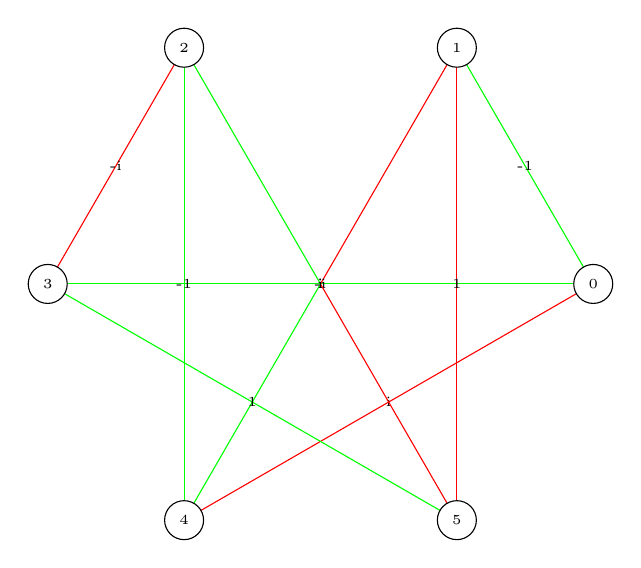
\begin{tikzpicture}
        \tikzstyle{every node}=[font=\tiny]
        \draw [style=thin, color=green] (3.464101615137755,0.0) to (2.5980762113533165,1.5);
\draw [style=thin, color=green] (2.5980762113533165,1.5) to (1.7320508075688779,3.0);
\node [style=circle, draw=none] at (2.5980762113533165,1.5) {-1};
\draw [style=thin, color=green] (3.464101615137755,0.0) to (0.0,2.1211504774498138e-16);
\draw [style=thin, color=green] (0.0,2.1211504774498138e-16) to (-3.464101615137755,4.2423009548996277e-16);
\node [style=circle, draw=none] at (0.0,2.1211504774498138e-16) {i};
\draw [style=thin, color=red] (3.464101615137755,0.0) to (0.8660254037844379,-1.4999999999999998);
\draw [style=thin, color=red] (0.8660254037844379,-1.4999999999999998) to (-1.732050807568879,-2.9999999999999996);
\node [style=circle, draw=none] at (0.8660254037844379,-1.4999999999999998) {i};
\draw [style=thin, color=red] (1.7320508075688779,3.0) to (-5.551115123125783e-16,2.220446049250313e-16);
\draw [style=thin, color=green] (-5.551115123125783e-16,2.220446049250313e-16) to (-1.732050807568879,-2.9999999999999996);
\node [style=circle, draw=none] at (-5.551115123125783e-16,2.220446049250313e-16) {-i};
\draw [style=thin, color=red] (1.7320508075688779,3.0) to (1.7320508075688765,-8.881784197001252e-16);
\draw [style=thin, color=red] (1.7320508075688765,-8.881784197001252e-16) to (1.7320508075688752,-3.0000000000000018);
\node [style=circle, draw=none] at (1.7320508075688765,-8.881784197001252e-16) {1};
\draw [style=thin, color=red] (-1.7320508075688767,3.0000000000000004) to (-2.598076211353316,1.5000000000000004);
\draw [style=thin, color=red] (-2.598076211353316,1.5000000000000004) to (-3.464101615137755,4.2423009548996277e-16);
\node [style=circle, draw=none] at (-2.598076211353316,1.5000000000000004) {-i};
\draw [style=thin, color=green] (-1.7320508075688767,3.0000000000000004) to (-1.7320508075688779,4.440892098500626e-16);
\draw [style=thin, color=green] (-1.7320508075688779,4.440892098500626e-16) to (-1.732050807568879,-2.9999999999999996);
\node [style=circle, draw=none] at (-1.7320508075688779,4.440892098500626e-16) {-1};
\draw [style=thin, color=green] (-1.7320508075688767,3.0000000000000004) to (-7.771561172376096e-16,-6.661338147750939e-16);
\draw [style=thin, color=red] (-7.771561172376096e-16,-6.661338147750939e-16) to (1.7320508075688752,-3.0000000000000018);
\node [style=circle, draw=none] at (-7.771561172376096e-16,-6.661338147750939e-16) {i};
\draw [style=thin, color=green] (-3.464101615137755,4.2423009548996277e-16) to (-0.8660254037844398,-1.5000000000000007);
\draw [style=thin, color=green] (-0.8660254037844398,-1.5000000000000007) to (1.7320508075688752,-3.0000000000000018);
\node [style=circle, draw=none] at (-0.8660254037844398,-1.5000000000000007) {1};
\node [style=circle, fill=white, draw=black] (0) at (3.464101615137755,0.0) {0};
\node [style=circle, fill=white, draw=black] (1) at (1.7320508075688779,3.0) {1};
\node [style=circle, fill=white, draw=black] (2) at (-1.7320508075688767,3.0000000000000004) {2};
\node [style=circle, fill=white, draw=black] (3) at (-3.464101615137755,4.2423009548996277e-16) {3};
\node [style=circle, fill=white, draw=black] (4) at (-1.732050807568879,-2.9999999999999996) {4};
\node [style=circle, fill=white, draw=black] (5) at (1.7320508075688752,-3.0000000000000018) {5};
\end{tikzpicture}
\end{document}